% Options for packages loaded elsewhere
\PassOptionsToPackage{unicode}{hyperref}
\PassOptionsToPackage{hyphens}{url}
%
\documentclass[
]{article}
\usepackage{lmodern}
\usepackage{setspace}
\usepackage{amssymb,amsmath}
\usepackage{ifxetex,ifluatex}
\ifnum 0\ifxetex 1\fi\ifluatex 1\fi=0 % if pdftex
  \usepackage[T1]{fontenc}
  \usepackage[utf8]{inputenc}
  \usepackage{textcomp} % provide euro and other symbols
\else % if luatex or xetex
  \usepackage{unicode-math}
  \defaultfontfeatures{Scale=MatchLowercase}
  \defaultfontfeatures[\rmfamily]{Ligatures=TeX,Scale=1}
\fi
% Use upquote if available, for straight quotes in verbatim environments
\IfFileExists{upquote.sty}{\usepackage{upquote}}{}
\IfFileExists{microtype.sty}{% use microtype if available
  \usepackage[]{microtype}
  \UseMicrotypeSet[protrusion]{basicmath} % disable protrusion for tt fonts
}{}
\makeatletter
\@ifundefined{KOMAClassName}{% if non-KOMA class
  \IfFileExists{parskip.sty}{%
    \usepackage{parskip}
  }{% else
    \setlength{\parindent}{0pt}
    \setlength{\parskip}{6pt plus 2pt minus 1pt}}
}{% if KOMA class
  \KOMAoptions{parskip=half}}
\makeatother
\usepackage{xcolor}
\IfFileExists{xurl.sty}{\usepackage{xurl}}{} % add URL line breaks if available
\IfFileExists{bookmark.sty}{\usepackage{bookmark}}{\usepackage{hyperref}}
\hypersetup{
  pdftitle={Evaluation of exotic maize hybrids for heat stress tolerance in Kailali, Nepal},
  pdfauthor={Prachi Bista,1; Deependra Dhakal,1,},
  pdfkeywords={Hybrid; Anthesis; Heat units; Heat tolerance; Silk emergence; Anthesis silking interval},
  hidelinks,
  pdfcreator={LaTeX via pandoc}}
\urlstyle{same} % disable monospaced font for URLs
\usepackage[top=0.85in,left=1in,footskip=0.75in,marginparwidth=2in]{geometry}
\usepackage{longtable,booktabs}
% Correct order of tables after \paragraph or \subparagraph
\usepackage{etoolbox}
\makeatletter
\patchcmd\longtable{\par}{\if@noskipsec\mbox{}\fi\par}{}{}
\makeatother
% Allow footnotes in longtable head/foot
\IfFileExists{footnotehyper.sty}{\usepackage{footnotehyper}}{\usepackage{footnote}}
\makesavenoteenv{longtable}
\setlength{\emergencystretch}{3em} % prevent overfull lines
\providecommand{\tightlist}{%
  \setlength{\itemsep}{0pt}\setlength{\parskip}{0pt}}
\setcounter{secnumdepth}{5}

% use Unicode characters - try changing the option if you run into troubles with special characters (e.g. umlauts)
\usepackage[utf8]{inputenc}

% clean citations
\usepackage{cite}

% hyperref makes references clicky. use \url{www.example.com} or \href{www.example.com}{description} to add a clicky url
\usepackage{nameref,hyperref}

% line numbers
\usepackage[right]{lineno}

% % improves typesetting in LaTeX
% \usepackage{microtype}
% \DisableLigatures[f]{encoding = *, family = * }

% text layout - change as needed
\raggedright
\setlength{\parindent}{0.5cm}
\textwidth 6.50in % \textwidth 5.25in
\textheight 8.75in % \textheight 8.75in

% use adjustwidth environment to exceed text width (see examples in text)
\usepackage{changepage}

% adjust caption style
\usepackage[aboveskip=1pt,labelfont=bf,labelsep=period,singlelinecheck=off]{caption}

% remove brackets from references
\makeatletter
\renewcommand{\@biblabel}[1]{\quad#1.}
\makeatother

% % headrule, footrule and page numbers
% \usepackage{lastpage,fancyhdr,graphicx}
% \usepackage{epstopdf}
% \pagestyle{myheadings}
% \pagestyle{fancy}
% \fancyhf{}
% \rfoot{\thepage/\pageref{LastPage}}
% \renewcommand{\footrule}{\hrule height 1pt \vspace{2mm}}
% \fancyheadoffset[L]{2.25in}
% \fancyfootoffset[L]{2.25in}

% use \textcolor{color}{text} for colored text (e.g. highlight to-do areas)
\usepackage{color}

% define custom colors (this one is for figure captions)
\definecolor{Gray}{gray}{.25}

% this is required to include graphics
\usepackage{graphicx}

% use if you want to put caption to the side of the figure - see example in text
\usepackage{sidecap}

\newcommand{\blandscape}{\begin{landscape}}
\newcommand{\elandscape}{\end{landscape}}

\usepackage{bm} % for supporting bold math fonts
\usepackage{siunitx}
\usepackage{moreverb}
\usepackage{booktabs}
\usepackage{longtable}
\usepackage{array}
\usepackage{multirow}

% use for have text wrap around figures
\usepackage{wrapfig}
\usepackage[pscoord]{eso-pic}
\usepackage[fulladjust]{marginnote}
\reversemarginpar

\usepackage{float}
\usepackage{colortbl}
\usepackage{pdflscape}
\usepackage{tabu}
\usepackage{threeparttable}
\usepackage{threeparttablex}
\usepackage[normalem]{ulem}
\usepackage{makecell}
\usepackage{xcolor}
\usepackage{tikz} % required for image opacity change
\usepackage[absolute,overlay]{textpos} % for text formatting
\usepackage{chemfig}

\newcommand\BibTeX{{\rmfamily B\kern-.05em \textsc{i\kern-.025em b}\kern-.08em
T\kern-.1667em\lower.7ex\hbox{E}\kern-.125emX}}
\sisetup{per-mode=symbol}

% this is to sort and place the reference in nice order
\DeclareRobustCommand{\firstsecond}[2]{#2}

% \bibliographystyle{plainnat}
\usepackage[numbers]{natbib}

% Added by CII
% \usepackage[format=hang,labelfont=bf,margin=0.5cm,justification=centering]{caption} # don't use bf
\usepackage[format=hang,margin=0.5cm,justification=centering]{caption}
\captionsetup{font=small,width=0.9\linewidth,labelfont=small,textfont={small}}
% End of CII addition

\usepackage{subcaption}
% \newcommand{\subfloat}[2][need a sub-caption]{\subcaptionbox{#1}{#2}}

% \captionsetup[sub]{font=footnotesize}
\captionsetup[subfigure]{font=small,labelfont=small,textfont=small}
\newlength{\cslhangindent}
\setlength{\cslhangindent}{1.5em}
\newenvironment{cslreferences}%
  {\setlength{\parindent}{0pt}%
  \everypar{\setlength{\hangindent}{\cslhangindent}}\ignorespaces}%
  {\par}

\title{Evaluation of exotic maize hybrids for heat stress tolerance in Kailali, Nepal}
\author{Prachi Bista\textsuperscript{$\dagger{}$,1} \and Deependra Dhakal\textsuperscript{$\dagger{}$,1,*}}
\date{2019-03-01}

\begin{document}
\maketitle
\begin{abstract}
Maize is a major food crop for Nepal, since time immemorial. Choice of planting material has been a critical aspect to ensuring good harvest, especially when end use are several. On one hand, grower should be careful to appropriately time the sowing and on the other, while making choice of maize hybrid for commercial cultivation, should consider growing heat tolerant hybrids when intended to tap into summer season crop. Testing and analysis of exotic maize hybrids targeted for high temperature condition adaptation are the subjects of current study. Standard fertilizer management with \SI{180}{\kg} N:\SI{60}{\kg} P:\SI{40}{\kg} K per hectare and soil moisture rating based irrigation scheduing will be practiced in growing 26 (including 3 known checks) hybrids in Dhangadhi-13, Kailali in an effort to understand yield and yield component traits as affected by heat stressed growing condition. It is suggested that the period extending from few days to months with high daily maximum temperature (\SIrange{40}{45}{\celsius}) that normally prevails over summer months in the study location are sufficient to induce heat associated physiological changes in maize crop and hence the broad effects in yield and component traits as well. Current study will delve into phenotypic characters that are known to have association to stress physiology and will aim to differentiate the tested maize genotypes for their tolerance to prevailing levels of heat stress.
\end{abstract}

\setstretch{2}
\textsuperscript{$\dagger{}$} These authors contributed equally to this work.

\textsuperscript{1} Gokuleshwor Agriculture and Animal Science College, Tribhuwan University, Kathmandu, Nepal

\textsuperscript{*} Correspondence: \href{mailto:ddhakal.rookie@gmail.com}{Deependra Dhakal \textless{}\href{mailto:ddhakal.rookie@gmail.com}{\nolinkurl{ddhakal.rookie@gmail.com}}\textgreater{}}

\newpage

\hypertarget{background}{%
\section{Background}\label{background}}

Maize ( \emph{Z. mays} L.) is a tall, monecious annual grass cultivated in \SI{956447}{\hectare} of land in Nepal fetching annual production of 2,713,635 tonnes (MoAD, 2077). It's cultivation, although a commonplace practice in Nepal, has been thriving in mostly traditional form despite claiming a major share as a staple food system. Consumption trend of Maize as of 2018 as suggested by the leading national maize research organization, NMRP, informs\footnote{\url{https://kathmandupost.com/money/2018/01/12/maize-output-to-hit-all-time-high-of-255-million-tonnes}} that 22.52 \% of the daily cereal uptake per capita (Hirai et al. 1993) is met with Maize. Since maize based agriculture system forms integral part of human food chain, while exhibiting prospects of continually increased contribution to dietary need supplementation, an honest step to mitigating long term food security in Nepal is investing resources to maize production and research.

A closer survey into food habit of past few years in Nepal suggests toward increasing meat consumption, especially that of poultry. Newer avenues for demand of maize as animal and poultry feed has opened. Furthermore, new types of maize-based products such as soups, vegetables and edible oils are in demand for use as food. While winter maize may be a promising technology intervention, longer growing season, extreme weather scenarios and inadequate irrigation infrastructures in major production pockets are the major hurdles to expansion of this technology.

Seasonal cultivation of maize in Nepal is generally scheduled differently for various agro-ecological zones. For instance, recommendation for optimal timing of planting in lower and higher mid-hill are is during summer second half of April/May and second half of March/April, respectively. For terai region, however, crop matures at relatively shorter growing period. Therefore, in areas with provision of proper drainage two harvests can be taken -- first planted in summer on second half of Feb/March and the second planted before onset of monsoon during second half of May/June season may.

Summer season maize plantation ensures early harvest and becomes a bridge to utilize fallow period between winter and monsoon season, the later being mostly dedicated to rice production. However, with gains come risk. Maize planted as summer crop in terai region of Nepal generally has to withstand scenario of extreme heat during vegetative-reproductive transitioning stage, unfortunately. Several studies have detailed on the ill consequences on yield components including reduced florets per ear, reduced number of viable kernel resulting due to kernel abortion, lesser silk extrusion, and reduced prolificacy of the crop that have gone through a period of high heat (Edreira et al. 2011). In contrast to biomass partitioning, severe effects were noted on final kernel number due to reduced overall biomass production under high temperature regimes (Echarte and Tollenaar 2006).

Effects of multifaceted events like climate change are being realized only recently in major cultivated crops including rice (Mukamuhirwa et al. 2019), lentil (Sehgal et al. 2017). Recent findings concerning effects of weather extremes, particularly during late vegetative and reproductive stages of the maize have underlined mechanisms that relate metabolism of upper body of crop to be detrimentally affected causing yield reduction (Zhao et al. 2016; Obata et al. 2015). Although touted a C4 plant having elaborate metabolic features that improve survival at high temperature and arid conditions, not unlike many other commercial crop maize requires a favorable growing period to realize good harvest. Shifting global climatic patterns are of major concern to countries of South Asia, notably Nepal, which traditionally have relied on low input use and mercy of good weather. As highlighted by Niyogi et al. (2015), current production systems are not sustainable and could be adversely impacted by extreme climate events in the near future.

Optimum yields occur when hybrids of suitable maturity duration and architecturally suited to dense population stand are chosen. In addition, exogenous sources of nitrogen fertilizer are generally applied and weed and insect control measures are generally recommended. Generally, hybrids are either early, medium or late maturing according to the amount of ``heat units'' that will be required for maturity.

Noting critical role of temperature regime during flowering and grain filling with heat stress causing severe reduction in economic yield (Barnabás, Jäger, and Fehér 2008), breeding for heat-tolerant cultivars is crucial to sustain crop production in the future. Genetic diversity analysis is imperative in crop improvement and can be studied through morphological, biochemical and molecular markers. Morphological characterization for genetic divergence among genotypes is considered an initial step (Chen et al. 2012).

\hypertarget{rationale}{%
\subsection{Rationale}\label{rationale}}

Heat stress greatly limits the productivity of maize in many regions. Knowledge of the genetic diversity of maize varieties along with information about traits conferring heat stress tolerance is necessary for generating effective breeding programs.

This study aims to elucidate the genetic mechanisms of heat tolerance under field conditions in maize and the genome regions contributing to natural variation.

Contribution of and effects on component traits in response to heat stress, differential expression of response on genotypes will be investigated in the current study. This will also extend the step of genotype characterization for more rigorous marker based genetic analysis.

\hypertarget{hypothesis}{%
\section{Hypothesis}\label{hypothesis}}

Null hypothesis that there is no significant difference among Maize genotypes will be tested. Likewise, contribution of component traits with potential impact on yield will be tested with yield response regression and pathway analysis.

\hypertarget{objectives}{%
\section{Objectives}\label{objectives}}

The objective of the research is to identify superior heat stress tolerant exotic hybrids for summer growth conditions in Kailali district of Nepal.

We also compare performance of national hybrids (selectively included as check) in terms of response to yield and associated components conditioned by prevailing summer heat.

\hypertarget{methodology}{%
\section{Methodology}\label{methodology}}

\hypertarget{site-selection}{%
\subsection{Site selection}\label{site-selection}}

The field experiment will be conducted in the research field of Matayari, Dhangadi-6, Kailali. The field is located at \(28^\circ 43' 48''\) N latitude and \(80^\circ 35' 57''\) E longitude at the altitude of 188 masl. The experimental site has tropical to sub-tropical climate with hot dry summer and cold winter. An account of meteorological data for past 3 years in the study site is depicted in Figure \ref{fig:climatology-matyari-dhangadhi}.

\begin{figure}

{\centering \subfloat[Cumulative monthly precipiation (from 2016 to 2019)\label{fig:climatology-matyari-dhangadhi1}]{\includegraphics[width=0.48\textwidth]{maize_genotype_trial_files/figure-latex/climatology-matyari-dhangadhi-1} }\subfloat[Daily maximum temperature (from 2017 to 2019)\label{fig:climatology-matyari-dhangadhi2}]{\includegraphics[width=0.48\textwidth]{maize_genotype_trial_files/figure-latex/climatology-matyari-dhangadhi-2} }

}

\caption{Daily weather (precipitation and temperature) of Dhangadhi-13, Kailali during few preceeding years of study}\label{fig:climatology-matyari-dhangadhi}
\end{figure}

Selected site is expected to beneficial due to its rich soil depth and cultivation friendly profile. Although, maize crop is said to perform well on a wide range of climatic conditions, its suitability to the study site is further corroborated with the following soil textural and composition attributes.

\begin{tabular}{ll}
\toprule
Feature & Condition\\
\midrule
Soil pH & 5\\
Soil texture & Clayey loam\\
Organic matter content & Moderate to high\\
O-horizon depth & > 15 cm\\
Slope & Low with delayed drainage\\
\bottomrule
\end{tabular}

For field preparation prior to planting, land will be made free of volunteer plants. Selected land will be deep ploughed twice followed by harrowing. Finally, prior to sowing rotary harrow or seed drill will be used to obtain a fine tilled bed.

\begin{table}[H]
\centering\begingroup\fontsize{10}{12}\selectfont

\begin{tabular}{>{\raggedright\arraybackslash}p{10em}>{\raggedright\arraybackslash}p{10em}lll}
\toprule
Collaborator & Location & Coordinates & Elevation & Climate\\
\midrule
\rowcolor{gray!6}  Unique Seed Company Private Limited & Dhangadhi-6 (Matyari), Kailali & \ang{28;43.48;}N, \ang{80;35.57;} E & 188m & Tropical\\
\bottomrule
\end{tabular}
\endgroup{}
\end{table}

\begin{itemize}
\tightlist
\item
  1 m distance between blocks
\item
  Dimension: 2.5 m × 4 m
\item
  Line sowing method: Continuous
\item
  Randomization design: Alpha lattice

  \begin{itemize}
  \tightlist
  \item
    Number of Replication (r) = 2
  \item
    Number of Blocks (b) = 4
  \item
    Number of blocks per replication (s) = 2
  \item
    Number of treatments per block (k) = 13
  \end{itemize}
\end{itemize}

\hypertarget{field-design-and-layout}{%
\subsection{Field design and layout}\label{field-design-and-layout}}

Trial was set on alpha lattice design with two replicates. Gross plot area for for each of the 52 plots was \SI{10}{\metre\squared}.

\begin{center}\includegraphics[width=0.98\linewidth]{maize_genotype_trial_files/figure-latex/alpha-layout-1} \end{center}

\hypertarget{interculture-management}{%
\subsection{Interculture management}\label{interculture-management}}

Spacing: Row to row \SI{60}{\centi\metre} and plant to plant \SIrange{20}{25}{\centi\metre}.

Fertilizer: Maize hybrids are responsive to nutrients applied either through organic or inorganic sources. The rate of nutrient application depends mainly on soil nutrient status/balance and cropping system. For obtaining desirable yield 180:60:40 kg NPK/ha with minimum 2 split dose of nitrogen should be followed. As the number of split of N increase the crop yield will increase accordingly.

Weeding: two hand weeding at 20 to 25 days after sowing and 40 to 45 days of sowing is necessary to control weed. Atrazine 1 to 2 manual weeding was followed as according to field condition. Pre-emergence application of Atrazine at the rate of \SIrange{1.0}{1.5}{\kg AI \per\hectare} in \SI{600}{\liter} water will be very effective in control of wide range of annual and broad leaf weeds.

Irrigation: Sufficient moisture should be available in soil during seed sowing, if not immediate irrigation should be given. Irrigation should be followed as according to the soil and climatic condition.

\hypertarget{data-collection-method}{%
\subsection{Data collection method}\label{data-collection-method}}

Data collection was followed as according to CIMMYT field book, days to flower (male and female), plant height, ear height, field weight, moisture, cob aspect and plant aspect were mainly considered.

\hypertarget{observations}{%
\subsection{Observations}\label{observations}}

\begin{enumerate}
\def\labelenumi{\arabic{enumi}.}
\item
  Days to Male Flowering: Record number of days from seed sowing to date of flowering of tassel (pollen shedding) in 50\% of plants in plot.
\item
  Days to Female Flowering: Record number of days from seed sowing to date of appearance of silk in 50\% of plants in plot.
\item
  Anthesis Silking interval (ASI): It is the difference of days from female flowering to the male flowering.
\item
  Plant height: It is the height of plant from base of the plant to the base of lower tassel branch. It should be collected form minimum 5 representative plants from plot.
\item
  Ear height: Height from base of the plant to the base of top most cob.
\end{enumerate}

\begin{figure}

{\centering \subfloat[Ear height\label{fig:maize-ear-height1}]{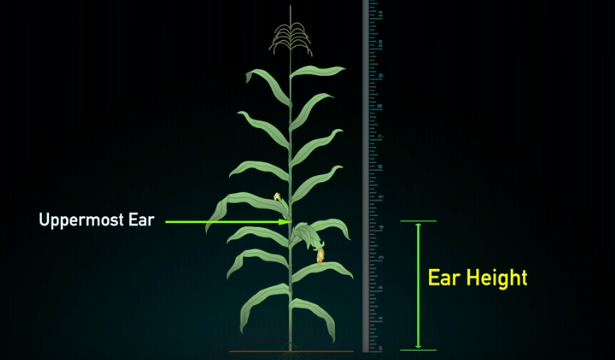
\includegraphics[width=0.48\textwidth]{./images/maize_ear_height} }\subfloat[Plant height\label{fig:maize-ear-height2}]{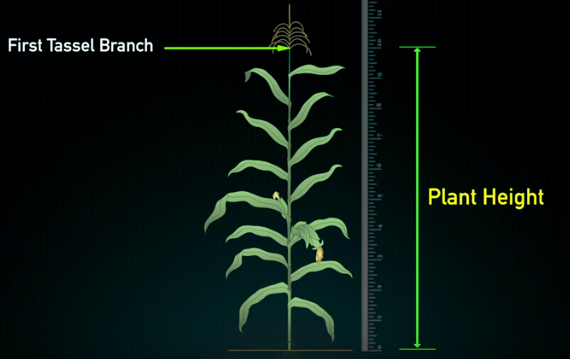
\includegraphics[width=0.48\textwidth]{./images/maize_height} }

}

\caption{Recording heights in Maize}\label{fig:maize-ear-height}
\end{figure}

\begin{enumerate}
\def\labelenumi{\arabic{enumi}.}
\setcounter{enumi}{5}
\item
  Field weight: Total weight of the dehusked cob during harvesting at field.
\item
  Number of plant and cob: Count the number of plants in whole plot during harvesting and total number of cobs from whole plot. It will help to find the prolifically and barren plants in plot.
\item
  Cob length: It is the length of cob from base to the tip of cob.
\item
  Cob circumference: It is the girth of the average sampled 5 cobs from middle part of cob. Cob diameter can also be measured by using vernier caliper from middle portion of cob.
\end{enumerate}

\begin{enumerate}
\def\labelenumi{\arabic{enumi}.}
\setcounter{enumi}{9}
\item
  Number of rows per cob: It is the number of rows presented in average sampled cob.
\item
  Number of grain per row: It is average number of grains presented in rows from sampled cobs.
\item
  Lodging: Number of plants fallen in ground should be counted. Plants fall from stem below cob are considered as stem lodging and if plants fall from ground (root) are counted as rood lodging.
\item
  Moisture: Several sampled cobs were selected and grain from middle portion of cob was taken at the time of harvesting when field weight is taken. Moisture was converted into 12.5\% for final data analysis.
\item
  Plant aspect: Complete visual score given by breeder to the overall plant performance of a variety. It incorporate major traits such as:
\end{enumerate}

\begin{itemize}
\tightlist
\item
  Ear position
\item
  Plant architecture
\item
  Tassel characteristics
\item
  Disease prevalence
\end{itemize}

It is recorded prior to the onset of crop senescence. It is scored from 1 to 5 scale;
- 1 represent excellent plant type, good yield potential, crop uniformity, lower ear position, vigorous, good stalk strength.
- 5 represent poor plant type, low yield, lodging, diseased, discoloured leaves and poor tassel exertion.

\begin{enumerate}
\def\labelenumi{\arabic{enumi}.}
\setcounter{enumi}{14}
\tightlist
\item
  Ear aspect: Ear aspect id the composite visual score given by breeders to the overall yield performance of the variety. It include key traits such as:
\end{enumerate}

\begin{itemize}
\tightlist
\item
  Yield
\item
  Ear rot
\item
  Texture
\item
  Ear uniformity
\item
  Grain filling
\item
  Cob covering
\item
  Ear symmetry
\end{itemize}

It is recorded just after cob harvesting and scored as 1 to 5:
- 1 represent excellent ear type, flint texture, disease free, large straight uniform rows.
- 5 represent poor ear type, small, rotten, non-uniform rows.

\begin{enumerate}
\def\labelenumi{\arabic{enumi}.}
\setcounter{enumi}{15}
\tightlist
\item
  Texture: maize grains can be differentiated into 4 texture group on the basis of their grain appearance:
\end{enumerate}

\begin{itemize}
\tightlist
\item
  1: flint,
\item
  2: semi flint,
\item
  3: semi dent
\item
  4: dent
\end{itemize}

\begin{figure}

{\centering 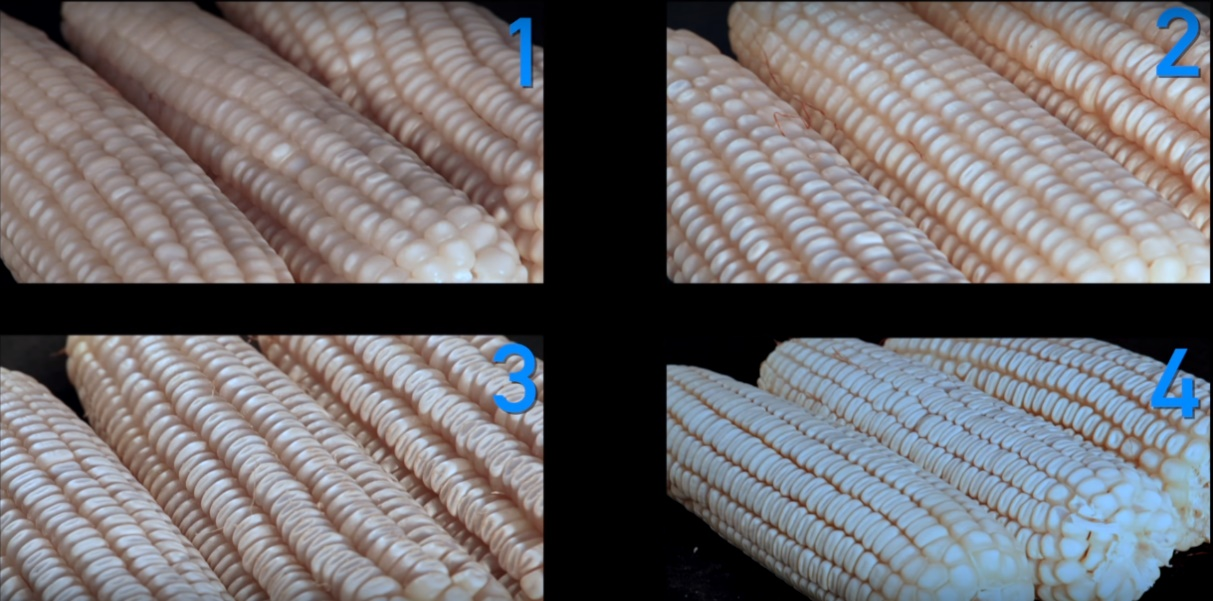
\includegraphics[width=0.6\linewidth]{./images/maize_texture} 

}

\caption{Scoring of grain texture in maize}\label{fig:maize-texture}
\end{figure}

Grain texture is recorded at harvest from all entry of trials.

\hypertarget{data-analysis}{%
\subsection{Data analysis}\label{data-analysis}}

Field observation data will be recorded in a field book for standing crop, soil parameters and post-harvest crop attributes. The field book will be transcribed to a database sheet, possibly using MSExcel software. Exploratory as well as inferential analysis will be carried out using open source application META-R.

\hypertarget{deliverables}{%
\section{Deliverables}\label{deliverables}}

\hypertarget{expected-outcomes}{%
\section{Expected outcomes}\label{expected-outcomes}}

\hypertarget{timeline}{%
\section{Timeline}\label{timeline}}

\begin{itemize}
\tightlist
\item
  Project started: March 1, 2020
\item
  Project end: February 28, 2021
\end{itemize}

\begin{figure}[H]

{\centering \includegraphics[width=0.75\textwidth]{maize_genotype_trial_files/figure-latex/timeline-1} 

}

\caption{Gantt chart of research showing estimated time periods for each activity}\label{fig:timeline}
\end{figure}

\hypertarget{budget}{%
\section{Budget}\label{budget}}

\renewcommand*{\arraystretch}{0.75}
\setlength{\baselineskip}{0.5\baselineskip}

\begin{longtable}{r>{\raggedright\arraybackslash}p{24em}r}
\toprule
SN & Particulars & Amount(NRs)\\
\midrule
\rowcolor{gray!6}  1 & Land preparation & 4000\\
2 & Soil sampling and analysis & 2500\\
\rowcolor{gray!6}  3 & Laying out of field (Nylon rope, plastic rope, staking bars, pegs, tags, tape, polythene bags, gunny bags) & 2000\\
4 & Organic manure and chemical fertilizers & 1415\\
\rowcolor{gray!6}   & Urea, DAP, Muriate of Potash and organic manure & \\
\addlinespace
5 & Seed sowing and bird proofing & 4000\\
\rowcolor{gray!6}  6 & Intercultural operations & 9500\\
 & Irrigation, weeding, fencing and guarding against herbivores and birds & \\
\rowcolor{gray!6}  7 & Plant protection spray against borer and small insects and fungal microbes (twice, at least) & 1500\\
8 & Travel expenditure & 5000\\
\addlinespace
\rowcolor{gray!6}  9 & Harvesting and threshing & 9000\\
 & Packing and bagging equipments, transportation, winnowing, grading & \\
\rowcolor{gray!6}  10 & Stationary and printing(labelling tags, observation entry sheets, design layout) & 2000\\
11 & Printing and reporting of manuscript drafts and revisions & 5000\\
\rowcolor{gray!6}   & Total & 45915\\
\bottomrule
\end{longtable}

\hypertarget{bibliography}{%
\section*{Bibliography}\label{bibliography}}
\addcontentsline{toc}{section}{Bibliography}

\hypertarget{refs}{}
\begin{cslreferences}
\leavevmode\hypertarget{ref-barnabas2008effect}{}%
Barnabás, Beáta, Katalin Jäger, and Attila Fehér. 2008. ``The Effect of Drought and Heat Stress on Reproductive Processes in Cereals.'' \emph{Plant, Cell \& Environment} 31 (1): 11--38.

\leavevmode\hypertarget{ref-chen2012characterization}{}%
Chen, Junping, W Xu, Jeffrey Velten, Zhanguo Xin, and John Stout. 2012. ``Characterization of Maize Inbred Lines for Drought and Heat Tolerance.'' \emph{Journal of Soil and Water Conservation} 67 (5): 354--64.

\leavevmode\hypertarget{ref-echarte2006kernel}{}%
Echarte, Laura, and Matthijs Tollenaar. 2006. ``Kernel Set in Maize Hybrids and Their Inbred Lines Exposed to Stress.'' \emph{Crop Science} 46 (2): 870--78.

\leavevmode\hypertarget{ref-edreira2011heat}{}%
Edreira, JI Rattalino, E Budakli Carpici, D Sammarro, and Maria Elena Otegui. 2011. ``Heat Stress Effects Around Flowering on Kernel Set of Temperate and Tropical Maize Hybrids.'' \emph{Field Crops Research} 123 (2): 62--73.

\leavevmode\hypertarget{ref-hirai1993food}{}%
Hirai, Kazuko, Jonko Nakayama, Mitsuko Sonoda, Yoshimi Ohno, Yoshinobu Okuno, Kumiko Nagata, Toshihide Tamura, Hem N Sakya, and Mathura P Shrestha. 1993. ``Food Consumption and Nutrient Intake and Their Relationship Among Nepalese.'' \emph{Nutrition Research} 13 (9): 987--94.

\leavevmode\hypertarget{ref-mukamuhirwa2019concurrent}{}%
Mukamuhirwa, Alphonsine, Helena Persson Hovmalm, Hans Bolinsson, Rodomiro Ortiz, Obedi Nyamangyoku, and Eva Johansson. 2019. ``Concurrent Drought and Temperature Stress in Rice---a Possible Result of the Predicted Climate Change: Effects on Yield Attributes, Eating Characteristics, and Health Promoting Compounds.'' \emph{International Journal of Environmental Research and Public Health} 16 (6): 1043.

\leavevmode\hypertarget{ref-niyogi2015crop}{}%
Niyogi, Dev, Xing Liu, Jeff Andresen, Yang Song, Atul K Jain, Olivia Kellner, Eugene S Takle, and Otto C Doering. 2015. ``Crop Models Capture the Impacts of Climate Variability on Corn Yield.'' \emph{Geophysical Research Letters} 42 (9): 3356--63.

\leavevmode\hypertarget{ref-obata2015metabolite}{}%
Obata, Toshihiro, Sandra Witt, Jan Lisec, Natalia Palacios-Rojas, Igor Florez-Sarasa, Salima Yousfi, Jose Luis Araus, Jill E Cairns, and Alisdair R Fernie. 2015. ``Metabolite Profiles of Maize Leaves in Drought, Heat, and Combined Stress Field Trials Reveal the Relationship Between Metabolism and Grain Yield.'' \emph{Plant Physiology} 169 (4): 2665--83.

\leavevmode\hypertarget{ref-sehgal2017effects}{}%
Sehgal, Akanksha, Kumari Sita, Jitendra Kumar, Shiv Kumar, Sarvjeet Singh, Kadambot HM Siddique, and Harsh Nayyar. 2017. ``Effects of Drought, Heat and Their Interaction on the Growth, Yield and Photosynthetic Function of Lentil (Lens Culinaris Medikus) Genotypes Varying in Heat and Drought Sensitivity.'' \emph{Frontiers in Plant Science} 8: 1776.

\leavevmode\hypertarget{ref-zhao2016difference}{}%
Zhao, Feiyun, Dayong Zhang, Yulong Zhao, Wei Wang, Hao Yang, Fuju Tai, Chaohai Li, and Xiuli Hu. 2016. ``The Difference of Physiological and Proteomic Changes in Maize Leaves Adaptation to Drought, Heat, and Combined Both Stresses.'' \emph{Frontiers in Plant Science} 7: 1471.
\end{cslreferences}

\end{document}
